\chapter{Atacul Meltdown}

Meltdown, descoperit în 2017, este un atac care permite citirea întregii
memorii de sistem (inclusiv a datelor personale și a parolelor), în ciuda
mecanismele de protecție care asigură izolarea memoriei kernel față de cea a unui
utilizator neprivilegiat. Atacul creează un canal de comunicare ascuns, pe baza
efectelor secundare ale \emph{Out-of-Order Execution}. Astfel, vulnerabilitatea
depinde doar de tipul procesorului pe care rulează sistemul și este independent
de software, sau tipul sistemului de operare. La momentul apariției Meltdown
afecta orice utilizator al unui procesor modern de tip \emph{Intel} produse 
începând cu 2011, și posibil alte mărci. Atacul a fost mitigat prin intermediul
unor patch-uri software pe toate sistemele mari de operare (Windows, Linux, 
Android, IOS, etc.) \cite{meltdown2018}.

În acest capitol vor fi prezentate particularitățile atacului, modul în care a
fost mititgat și modul în care poate fi reprodus.

\section{Descrierea Atacului}

Meltdown se bazează pe executarea intenționată a unor instrucțiuni care produc
excepții prin natura lor (accesare unor zone interzise de memorie), dar care la
nivel microarhitectural sunt executate, iar datele sunt accesate. Prin
intermediul \emph{Out-of-Order Execution} și a instrucțiunilor tranzitorii,
datele respective sunt folosite pentru a produce o schimbare masurabilă la
nivel arhitectural și anume, în cache-ul procesorului. Prin tratarea excepțiile
ridicate de sistemul de operare în urma instrucțiunilor ilegale și folosind
unul dinte atacurile documentate asupra memoriei cache, precum \emph{FLUSH and
RELOAD}, creăm un canal secundar de comunicare prin care atacatorul capătă
acces la date în mod neprivilegiat.

\subsection{Structura Memoriei Virtuale în Cadrul unui Proces}

Pentru înțelegerea atacului este important de înțeles cum arată spațiul
memoriei virtuale la nivelul fiecărui proces. Kernelul are nevoie de acces la
toată memoria. Astfel toată memoria fizică este mapată în kernel la o anumită
adresă. De asemenea, spațiul de memorie alocat unui proces este împărțit între
zona utilizatorului și zona de kernel. Kernelul administrează tabelele de
traducere a adreselor de memorie și veghează ca accesul utilizatorului să fie
restricționat doar la spațiile de memorie în care se află datale folosite de
programul curent. Astfel, în ciuda faptului că în cadrul procesului există
alocate adrese virtuale de memorie care corespund adresei fizice a kernelului,
acestea nu pot fi accesate fără privilegii speciale (determinate de
\emph{user/supervisor bit} vezi \ref{sec:virtual_memory} și figura
\ref{fig:vmem}) în cadrul rulării unui program în parametrii normali
\cite{kernel}. 

\begin{figure}[ht]
	\centering
	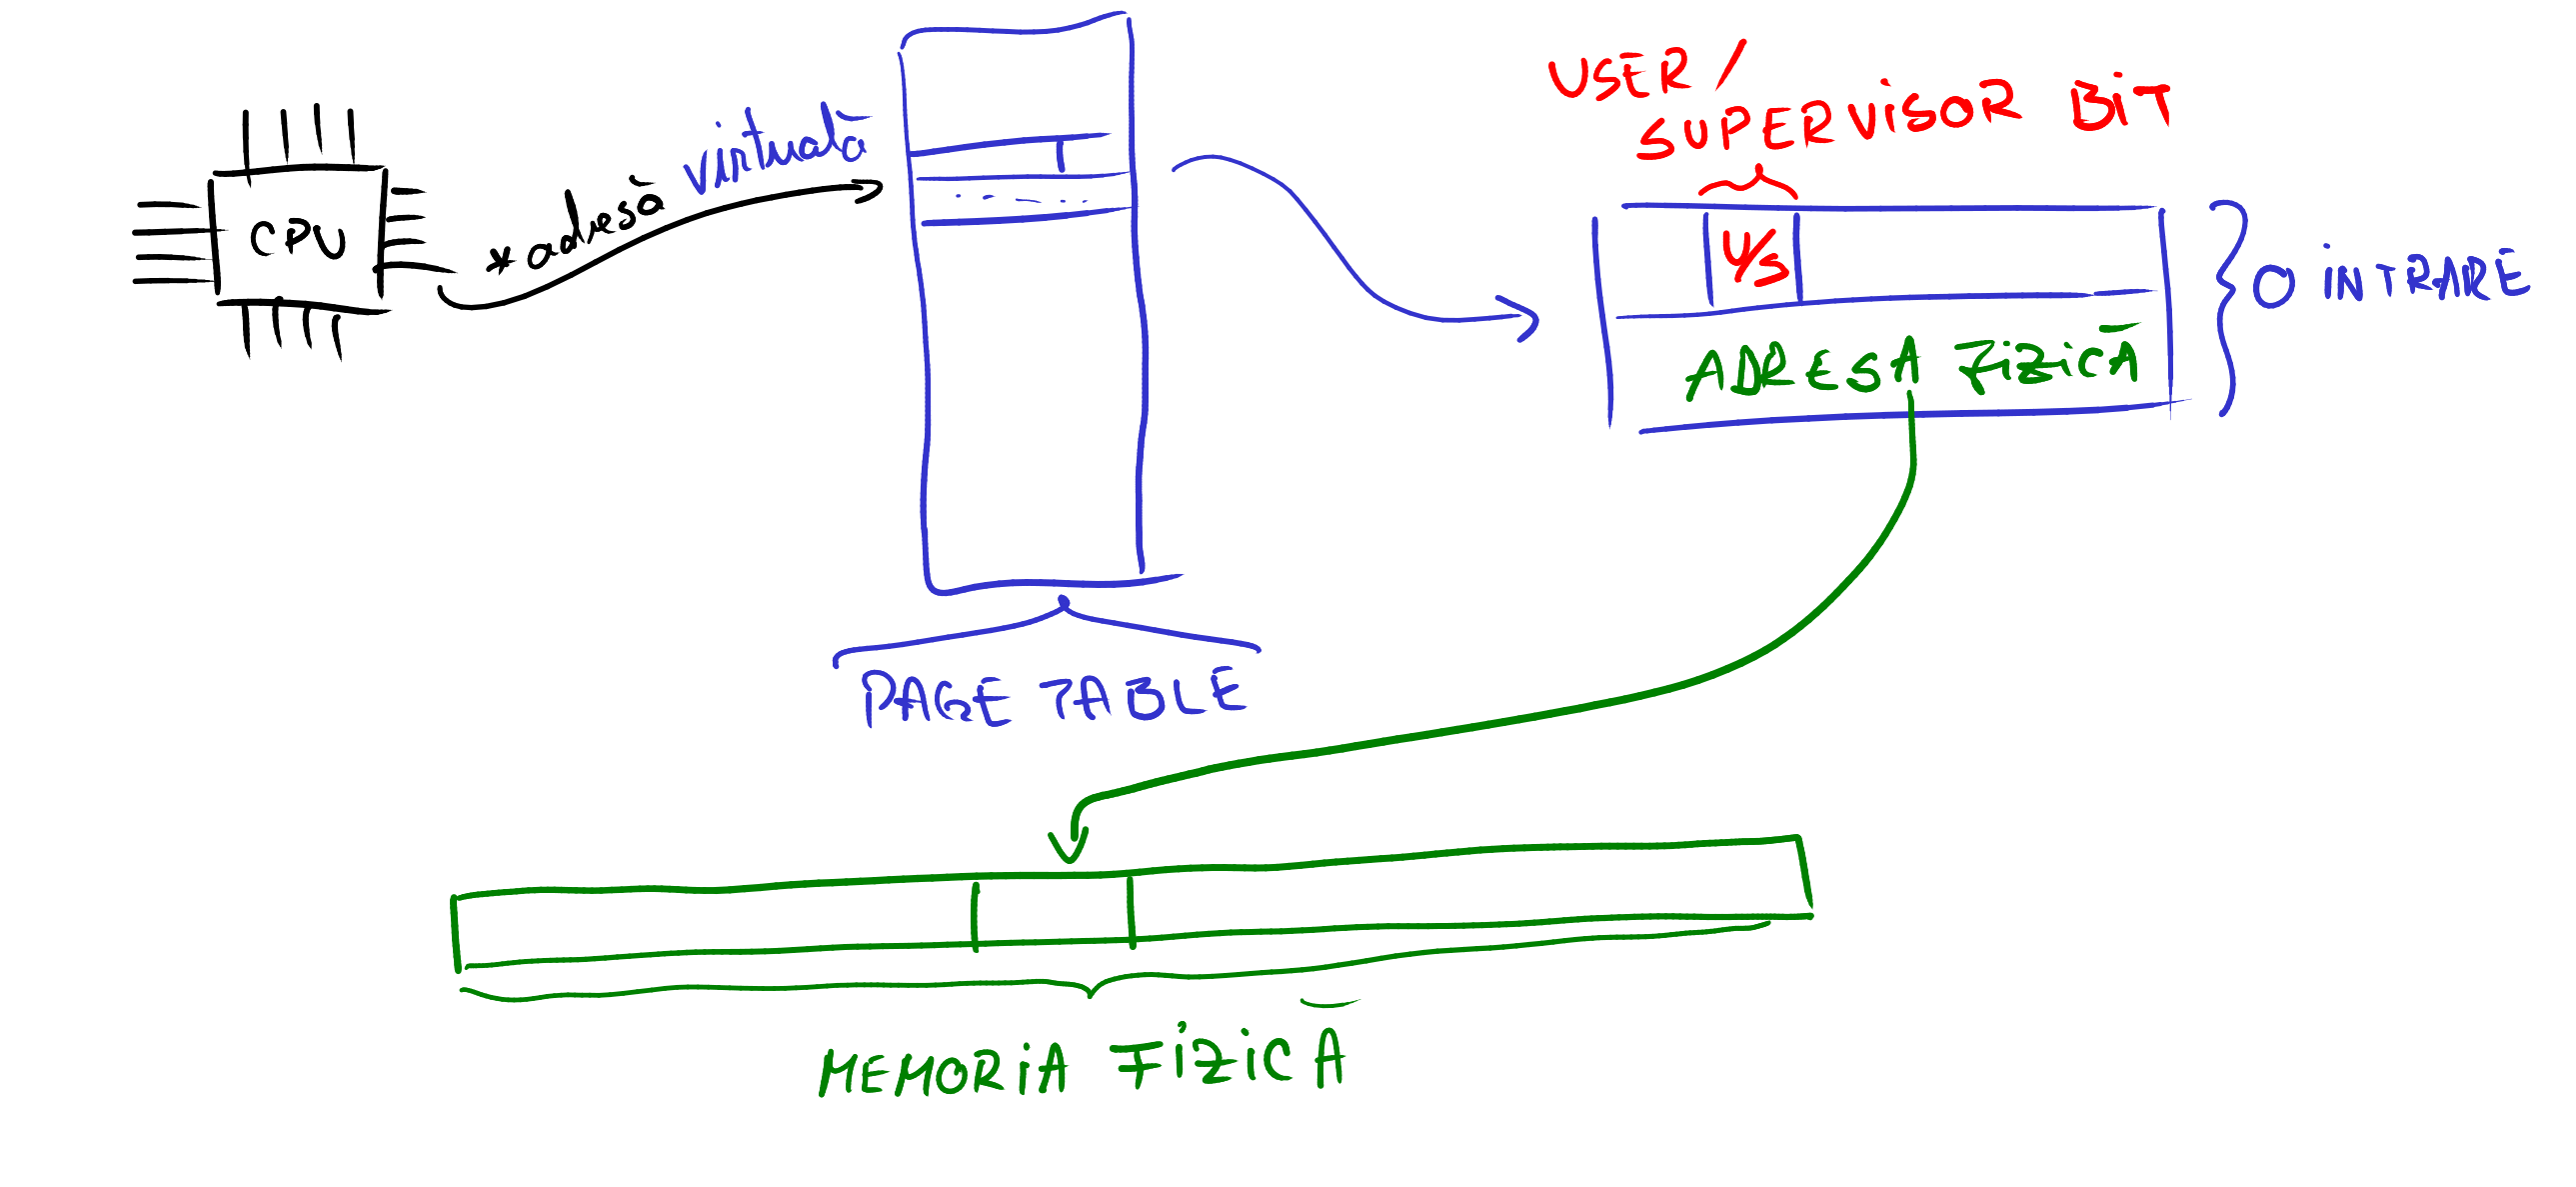
\includegraphics[width=0.9\textwidth]{images/vmem.png}
  \caption{Traducerea adresei virtuale în adresa fizică}
  \label{fig:vmem}
\end{figure}

La momentul descoperirii atacului, întreaga memorie fizică putea fi accesată
prin intermediul kernel-ului, fiind mapată direct în cadrul acestuia. Meltdown
reușește să ignore regulile stricte de separare dintre user și kernel și prin
intermediul acestei legături directe între kernel și restul memoriei poate citi
date fară drepturi asupra acestora. Mitigarea vulnerabilității a constat în
consolidarea mecanismelor de separarea dintre utilizatorul neprivilegiat și
kernel.

\subsection{Exectuarea Instrucțiunilor Tranzitorii}

Scopul atacului este de a accesa și citi date asupra cărora utilizatorul nu are
drepturi, așadar în cadrul atacului vom ținti acest tip de zone de memorie.
După cum am menționat în secțiunea \ref{sec:ooo_exec}, procesoarele moderne
execută adesea instrucțiunile într-o ordine diferită de cea în care apar
acestea în program. Există posibilitatea ca astfel de instrucțiuni să ruleze
înainte ca verificările asupra drepturilor de executare asupra acelei
instrucțiuni să fie finalizate. Să considerăm următoarea secvență de cod:

\begin{lstlisting}[language=c,caption=Executarea instrucțiunilor tranzitorii,
                   escapeinside={(*}{*)}]
   // declararea în prealabil a variabilelor
   int x;
   char kernel_data;

   // accesare kernel produce exceptie
   kernel_data = *kernel_data_addr; (*\label{lst:tranz_deref}*) 
   // instructiunile care urmeaza nu sunt niciodata executate la nivel macro

   // accesarea elementului din tabloul  duce la
   // încarcarea în cache a unei linii care include 
   // index-ul asociat valorii byte-u-lui citit din zona de kernel
   x = probe[kernel_data * 4096]; (*\label{lst:tranz_probe}*)
\end{lstlisting} \label{code:transient}

Se presupune că avem la cunoștință adresa unui secret stocat în zona de kernel
stocată în variabila \texttt{kernel\_data\_addr}. Execuția instrucțiunilor din
linia \ref{lst:tranz_deref} va duce la dereferentia adresei respective, ceea ce va produce un
\emph{Segmentation Fault}. Astfel, la nivel macro, prin intervenția sistemului
de operare, datele de la adresa respectivă nu vor fi accesate, conform
restricțiilor impuse de kernel asupra utilizatorului neprivilegiat.
Comportamentul astfel rezultat al programului este cel așteptat.

La nivel microarhitectural fluxul de execuție diferă. Verificarea drepturilor
de acces asupra unei zone de memorie au loc după accesarea acesteia. Din cauza
\emph{Out-of-Order Execution} și rulării relativ lentă a verificării
drepturilor de accesare, instrucțiunile care succed vor fi executate
speculativ. La nivel microarhitectural datele de la adresa
\texttt{kernel\_data\_addr} vor fi preluate și încărcate în variabila
\texttt{kernel\_data}. Ulterior, tabloul \texttt{probe} vă fi accesat la
index-ul corespunzător \texttt{kernel\_data}, iar pagina corespunzătoare acelei
valori vă fi încărcată în cache (linia \ref{lst:tranz_probe}). Rezultatele obținute vor fi
evident omise când dreptului de acces asupra adresei respective este invalidat,
iar starea registrilor vă trebui resetata la cea anterioara liniei \ref{lst:tranz_deref}. 

Din cauza unui bug în arhitectura majorității procesoarelor, datele încărcate
în cache-ul procesorului în cadrul executării speculative, rămân în cache chiar
și după resetarea stării microarhitecturale. Aceste \emph{Instrucțiuni
Tranzitorii} prin faptul că nu resetează starea cache-ului permit folosirea
tehnicilor specifice atacurilor cache pentru recuperarea secretului
\cite{meltdown2018}.

\subsubsection{Observație - Principiul Localității}\label{sec:locality}

Trebuie făcută o observație importantă pentru linia \ref{lst:tranz_probe}. În cadrul
instrucțiunii tranzitorii pe care vrem să o executăm am accesat tabloul
\texttt{probe} la index-ul $kernal\_data \times 4096$, în loc de
$kernel\_data$. Conform \emph{principiului localității}
\cite{denning2006locality}, când are loc un cache miss procesorul nu încarcă
doar 1 byte din memorie, ci multiplii bytes în funcție de dimensiunea liniilor
din cache (de obicei 64 de bytes). Rezultatul este că în momentul în care un
element \texttt{probe[k]} ar fi accesat, și el și elementele adiacente acestuia
ar fi încărcate în cache. Pentru a putea distinge ușor între elemente adiacente
vom folosi un multiplicator (în acest caz $4096$) mai mare decât dimensiunea 
tipică a unei linii de cache pentru ca accesarea a două elemente adiacente să nu
determine încărcarea în cache a unor blocuri cu zone comune.

\subsection{Gestionarea Excepțiilor}

Pentru a nu întrerupe fluxul de execuție și a putea interpreta datele rezultate
în urma \emph{Instrucțiunilor Tranzitorii} trebuie tratate execeptiile apărute
în mod natural. Conform lucrării de cercetare \cite{meltdown2018} avem două
variante: suprimarea sxcepțiilor și tratarea explicită a excepțiilor.

\subsubsection{Duplicarea Procesului}

O metodă trivială presupune duplicarea (\emph{forking}) procesului chiar înainte
de declanșarea excepției. Linia \ref{lst:tranz_deref} a codului ar fi astfel executata în procesul
copil, care va fi terminat de către sistemul de operarare. Efectele secundare 
apărute în urma execuției speculative pot fi apoi măsurate din procesul părinte
prin intermediul unui canal secundar (\emph{side-channel}), eg. memoria cache.

\subsubsection{Signal Handler}

O metodă alternativă este instalarea unui \emph{signal handler} care se
declanșează la apariția excepției corespunzătoare (eg. \emph{Segmentation Fault})
Astfel evităm terminarea programului de către sistemul de operare și reducând 
timpul de execuție necesar creării unui nou proces.

\subsubsection{Suprimarea Excepțiilor}

Putem de asemenea preveni declanșarea excepțiilor în totalitate. În cadrul
execuției speculative se pot executa instrucțiuni care nu s-ar executa în mod
normal din cauza unei predicții greșite a căii urmate de fluxul de instrucțiuni
în urma unei bifurcări. Astfel, deoarece la nivel macro instrucțiunile ilegale
nu vor fi executate, excepția nu va fi declanșată de sistemul de operare, chiar
dacă la nivel microarhitectural, liniile de cod au fost executate speculativ,
iar efectul secundar a avut loc. Această abordare implică antrenarea oracolului
de prezicere a bifurcărilor (\emph{branch predictor}) și va fi descris în
cadrul discuției despre \emph{Atacuri Spectre} \cite{spectre2019}.

\subsection{Trecerea din planul micro în planul macro}\label{sec:step_receive}

Ca urmare a gestionării excepțiilor, execuția programului continuă
neîntreruptă. În urma executării instrucțiunilor tranzitorii, la nivel
microarhitectural starea sistemului s-a schimbat, prin încărcarea în cache a
adresei accesate speculativ. Prin intermediul tehnicilor specifice atacurilor
asupra memoriei cache (descrise în secțiunea \ref{sec:atacuri_cache}) putem crea un
canal secret de comunicare (covert channel). Va fi prezentată inițial metoda de
transmitere a unui bit pe canalul secret, iar ulterior această metodă va fi
extinsă la transmiterea unui byte.

Pentru a transmite un bit se procedează în felul următor. Pentru transmiterea
de informație se executa o serie de instrucțiuni tranzitorii în urma cărora
zona de memorie dorita este încărcată în cache. Pentru citirea informației de
pe canalul ascuns este folosită tehnica \emph{FLUSH and RELOAD}
(\ref{sec:flush_reload}). Inițial se folosește instrucțiunea \texttt{clflush}
pentru eliberarea din cache (eviction) a adresei tintă, iar apoi se așteaptă
transmiterea unui bit de informație. După trecerea perioadei de timp se măsoară
timpul necesare accesării valorii de la adresa tintă. Dacă timpul de accesare
este mic (sub un prag stabilit anterior) îl clasificăm ca \emph{cache hit}. În
acest caz, constatăm că victima a accesat în fereastra de timp adresa de
memorie prin intermediul unei instrucțiuni tranzitorii, și a transmis atfel un
bit cu valoarea emph{1}. Dacă timpul de accesare este mare (peste pragul
stabilit anterior), clasificăm accesarea că un \emph{cache miss}. În acest caz,
victima nu a executat instrucțiunile tranzitorii corespunzătoare încărcării în
cache a valorii țintă, deci a transmis implicit un bit cu valoare \emph{0}.

Pentru transmiterea a 1 byte de date (dimensiunea corespunzătoare unui caracter
în format ASCII) se va proceda în felul următor. Conform secțiunii de cod din
\ref{code:transient}, pentru fiecare dintre cele 256 de valori posibilie pe
care le poate avea un byte de informație, se accesează o linie separată în
cache în mod speculativ prin intermediul unui set de instrucțiuni tranzitorii.
Pentru reconstruirea informației, atacatorul vă efectua atacul \emph{FLUSH and
RELOAD} pentru fiecare dintre cele 256 de zone posibile din cache. Inițial,
fiecare dintre cele \emph{256} de adrese trebuie eliminate din cache (se
folosește instrucțiunea \texttt{clflush}). În final, index-ul pentru care s-a
obținut un \emph{cache hit} va corespunde valorii byte-ului de informație
transmis prin canalulu secret (vezi figura \ref{fig:flush_reload}). În
particular, pentru array-ul \texttt{probe} se vă rula \emph{FLUSH and RELOAD}
pentru fiecare dintre \texttt{probe[i * 4096]} (cu $0 \leq i \leq 255$). Dacă
se obține un \emph{cache hit} pentru \texttt{probe[k * 4096]} (cu $0 \leq i \leq
255$), atunci pe canal s-a transmis valoarea \emph{k} \cite{meltdown2018}. 

\begin{figure}[ht]
	\centering
	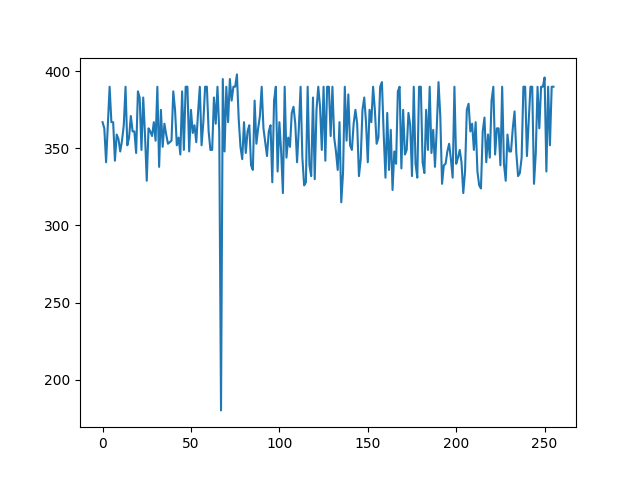
\includegraphics[width=0.9\textwidth]{images/flush_reload_hit.png}
  \caption{Recuperarea unui byte prin Flush \& Reload}
  \label{fig:flush_reload}
\end{figure}

Conform principilui localității (descris aici \ref{sec:locality}) vom mutiplica
valoarea secretului cu \emph{page-size} (în acest caz \emph{4KB}) pentru a
asigura o separare suficient de mare între adresele accesate din
\texttt{probe}. Astfel evităm scenariul în care în urma unei accesări, printre
valorile adiacente indicelui accesat, la un pas, sunt încărcate în cache și
valorile ale unori indici de interes. Astfel, tabloul \texttt{probe} va avea
dimensiunea de exact $256 \times 4096$ pentru pagini de \emph{4KB}.

\subsection{Scenariul și realizarea atacului Meltdown}

La momentul apariției, atacul Meltdown avea ca tintă orice fel de computer
personal, ori mașină virtuală în cloud. Se presupune că atacatorul nu dispune
de acces fizic asupra mașinilor atacate, dar poate executa orice fel de cod în mod
neprivilegiat, cu aceleași drepturi ca un utilzator obișnuit (fără drepturi de
root, ori administrator). Sistemul tintă este protejat de mecanisme considerate
\emph{state-of-the-art} la vremea respectivă (i.e. nu luăm în considerare
mecanismele de protecție apărute ulterior care au ca rezultat mitigarea
atacului, acestea fiind discutate în secțiunea \ref{sec:mitigare_meltdown}),
precum \emph{ASLR} și \emph{KASLR}. Sistemul dispune de asemenea de un
procesor care suportă \emph{Out-of-Order Execution}. Atacul nu se bazează pe
niciun fel de vulnerabilitate de tip software, exploatând doar hibe la nivel
hardware. Astfel, se presupune rularea unui sistem de operare fără probleme
cunoscute care pot fi abuzate pentru elevarea nivelului de privilegii. Ținta
atacatorului va fi orice tip de informație de valoare precum chei de acces,
parole, hash-uri, date personale, etc.

Atacul presupune obținerea adresei din kernel a secretului prin diferite
mecanisme (care nu reprezintă scopul acestei lucrări), ori ghicirea acesteia.
Ulterior se execută pașii descriși mai sus. În primă fază va trebui să se
execute un set de instrucțiuni alese special, care folosesc adresa tintă și se execută
în mod speculativ, devenind ulterior tranzitorii în urma
declanșării unei excepții. Între decodarea adresei virtuale în adresă fizică,
accesarea valorii corespunzătoarea și încărcarea în cache a liniei
aferente \emph{(1)}, și verificarea drepturilor de acces asupra zonei de
memorie conform drepturilor de utilizator și restricțiilor din tabela de
traducere \emph{(2)}, se produce un \emph{race condition}. În cazul în care
\emph{(1)} se execută mai rapid decât \emph{(2)} starea microarhitecturala va
fi modificată în modul dorit, iar abia apoi sistemul de operare va constata
accesul nepermis și va declanșa o excepție. Ajunși în acest punct, rolul
emițătorului este finalizat. Pentru receptarea mesajului se gestionează
excepția de tip \emph{Segmentation Fault} declanșată de sistemul de operare
(printr-una din metodele descrise anterior), iar apoi se folosește \emph{FLUSH
and RELOAD} pentru a recupera secretul (\ref{sec:step_receive}).

Acești trei pași determină obținerea unui byte din secret. Pentru obținerea
întregului secret se iterează prin toate adresele de memorie ale căror valoari
sunt de interes. În mod similar se poate descărca întreaga memorie fizică a 
sistemului tintă.

\section{Sisteme evaluate}

Conform particularităților atacului, orice sistem al cărui hardware este
vulnerabil va fi vulnerabil indiferent de software-ul care rulează (considerând
că patch-ul software nu este aplicat). Într-adevăr s-a constatat că atacul
poate dezvălui informații secrete ale unui utlizator neprivilegiat pe multiple 
sisteme utilizate la scară largă.

\subsection{Linux}

Meltdown a putut fi rulat pe multiple versiuni ale kernel-ului de Linux, de la
2.6.32 la 4.13.0, acestea mapând adresele kernelului în spațiul virtual al
oricărui proces neprivilegiat, bineînțeles cu restricțiile de acces aferente, acestea
fiind implementate corect în tabelele de traducere a adreselor \cite{meltdown2018}.

\subsection{Microsoft Windows}

Meltdown a putut fi rulat pe un sistem cu Windows 10, cu actualizările la zi,
chiar înainte de aplicarea patch-urilor. În ciuda modului diferit în care este
mapată memoria fizică și management-ului diferit al acesteia, majoritatea memoriei
fizice tot se poate citi prin intermediul atacului. Cercetătorii au putut citit 
întregul binar al kernelul-ului de Windows \cite{meltdown2018}.

\subsection{Android}

Deoarece Android-ul are la bază tot Kernel-ul de Linux, succesul atacului pe
această platforma depinde de procesorul instalat pe dispozitiv. Astfel în urma
testelor asupra unui Samsung Galaxy S7 rulând un Linux Kernel cu versiunea
3.18.14, atacul nu a avut succes pe asupra procesorului ARM Cortex A53, dar a
funcționat asupra celor marca Exynos dezvoltate de Samsung.

\subsection{Containere}

Tehnologiile de containerizare care împart între ele același kernel sunt și ele
vulnerabile. Meltdown poate fi rulat cu succes în containere Docker, LXC, sau
OpenVZ și s-a demonstrat că prin intermediul lui se pot extrage informații nu
numai din kernel, dar și din celelalte containere care rulează pe aceeași
mașină fizică. Rezultatul vine din cauză că fiecare container împarte kernel-ul
cu toate celelalte, așadar orice proces va avea încărcat în spațiul său virtual
de memorie întreagă memorie fizică a sistemului, prin intermediul kernel-ului
împărțit cu celelalte containere și procese care rulează pe același sistem.

\subsection{ARM și AMD}

În ciuda succesului pe arhitectura \emph{Intel} și pe câteva modele
\emph{Exynos}, atacul nu a putut fi executat cu succes pe procesoare
\emph{AMD}. \emph{AMD} susțin că acest rezultat se datorează unor diferențe
arhitecturale în comparație cu \emph{Intel} \cite{amd_response}. În cazul
\emph{ARM}, signrul procesor afectat ar fi modelul \emph{Cortex-A75}, conform
\cite{grisenthwaite2018cache}. Deoarece detaliile de implementare ale
microarhitecturilor nu sunt în general dezvăluite publicului larg nu se poate
determină cu exactitate ce a determinat aceste diferențe.

\section{Performanța}

Performanța atacului depinde de modul și eficiența cu care se câștigă
\emph{race condition}-ul. Indiferent de locația din memorie în care se află
datele dorite, s-a demonstrat că \emph{race condition}-ul poate fi câștigat,
dar diferențele de performanță sunt notabile.

\subsection{Secretul în cache}

Când datele sunt în imediata apropiere a procesorului (în cache-ul \emph{L1}),
\emph{race condition}-ul poate fi castigat cu ușurință. Astfel s-au obținut
performanțe ridicate de până la $582$ KB/s cu rata de eroare de până la
$0.003\%$ (Intel Core i7-8700K). O variantă mai lentă a atacului care reduce
eroarea la $0$ ajunge la viteze de $137$ KB/s \cite{meltdown2018}. 

În cazul în care secretul se află în cache-ul \emph{L3}, dar nu în cache-ul
\emph{L1}, \emph{race condition}-ul încă se poate căștiga des, dar viteza vă fi
mult mai mică, de până la $12.4$ KB/s, cu erori de până la $0.02 \%$
\cite{meltdown2018}.

\subsection{Secretul în afara cache-ului}

În acest caz câștigarea \emph{race condition}-ului este mai dificilă. S-au
observat rate de transimitere a datelor de sub $10$ B/s pe majoritatea
sistemelor. Aceste rezultate au putut fi îmbunătățite cu ajutorul a două
optimizări. Acestea presupun preîncărcarea zonelor de memorie din cache prin
intermediul unor thread-uri care rulează în paralel (conform
\cite{gruss2016prefetch}) și abuzând de implementarea cache-ului conform
principiului localitații (vezi \ref{sec:locality}) prin accesarea speculativă a
zonelor adiacente țintei, astfel încărcând în cache și adresa țintă.
Optimizările cresc viteza de citire până la $3.2$ KB/s \cite{meltdown2018}.

\section{Metode de mitigare}
\label{sec:mitigare_meltdown}

\subsection{Hardware}

Meltdown nu exploatează niciun defect de natură software, ci ocolește
restricțiile de acces prezente la nivel hardware prin intermediul 
execuției instrucțiunilor \emph{out-of-order}.

Considerând mecanismele exploatate în cadrul acestui atac, două contramăsuri
posibile ar fi eliminarea completă a \emph{out-of-order execution}, sau
serializarea instrucțiunilor care verifică permisiunile de acces și accesarea
propriu-zisă a zonei de memorie, pentru a evita executarea acestora în paralel.
Aceaste soluții nu ar fi fezabile întrucât impactul pe care l-ar aduce asupra
performanței este mult prea mare.

O soluție mai realistă ar fi separarea la nivel hardware a zonei utilizatorului
și a zonei Kernel printr-un \emph{bit} suplimentar care marchează activarea
acestui sistem. În cazul în care ar fi activat se impune ca adresele kernel-ului
să se regăsească în jumătatea superioară a memoriei, iar adresele
utilizatorului în jumătatea inferioară. Acest mecanism ar avea un impact
neglijabil asupra performanței, deoarece nivelul de permisiuni poate fi dedus
direct în adresa virtuală, astfel dreptul de acces putând fi confirmat sau
infirmat direct, fară accesări suplimentare ale tabelei de traducere.

\subsection{Software -- KAISER}

Deoarece rezolvarea problemelor prezente în hardware-ul aflat în prezent în
folosință este imposibil de implementat în practică, a trebuit găsită o soluție
de natură software. Meltdown poate avea loc deoarece adresele kernel sunt mapate
în spațiul procesului chiar dacă acestea rulează neprivilegiat. Adresele
virtuale mapate sunt legitime și corespund unor adrese fizice. Singurul
mecanism care limitează accesul unui utilizator oarecare în spațiul kernel-ului
constă în restricțiile prezente în tabelele de traducere a adreselor fiecărui
proces. Acest mecanism funcționează la nivel arhitectural, rezultatul final al
execuției fiind cel așteptat. La nivel microarhitectural, s-a demonstrat că
prin intermediul execuției instrucțiunilor într-o altă ordine, în mod
speculativ, se pot accesa din spațiul user-ului zone de memorie din kernel
înainte ca dreptul de acces să fie confirmat. Soluția naturală propusă a fost
utilizarea a două spații de memorie separate pentru fiecare proces: unul
dedicat utilizatorului în care kernel-ul nu este mapat, și unul dedicat
kernel-ului în care spațiul utilizatorului nu este mapat. Din diverse motive de
performanță și practicalitate, printre care faptul că nemaparea spațiului
utilizatorului în Kernel ar presupune rescrierea unor porțiuni considerabile
din Kernel, s-a ajuns la implementarea pe majoritatea sistemelor a unei soluții
bazate pe KAISER (\cite{gruss2017kaslr}) (în Kernel-ul de Linux aceasta poartă
numele de KPTI sau PTI -- \emph{Kernel Page-Table Isolation}).

KAISER a fost propus ca soluție pentru atacurile asupra \emph{Kernel Address
Space Layout Randomization} (KASLR) și presupune o metodă de separare a
spațiului kernel de spațiul utilizatorului. Acest mecanism de protecție are la
bază conceptul de spațiu de adrese fantomă (\emph{shadow address space}).
Astfel, în mod neprivilegiat adresele kernel nu sunt mapate, iar în mod
privilegiat adresele utilizatorului sunt mapate și vegheate de mecanismele de
securitate \emph{SMEP} și \emph{SMAP} care previn execuția codului unui
utilizator în spațiul kernel, sau posibile corupții ale memoriei. Schimbarea
între cele două contexte se face foarte ușor, prin aplicarea unei măști pe biți
asupra registrului \texttt{CR3}, în care se reține adresa tabelei de traducere
corespunzătoare contextului curent. Implementarea acestei soluții previne
atacul Meltdown, întrucât în modul de rulare neprivilegiat nu există adrese
virtuale care să corespunda unor zone sensibile din kernel. S-a demonstrat
că aceasta soluție are costuri de performanță neglijabile, în medie de $0.28\%$
\cite{gruss2017kaslr}.

\begin{figure}[ht]
	\centering
	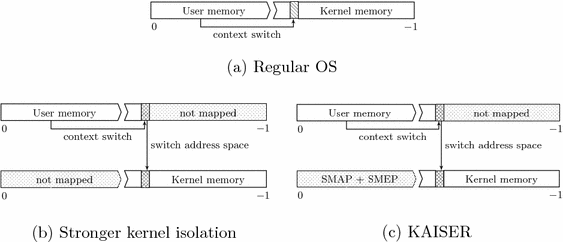
\includegraphics[width=0.9\textwidth]{images/shadowspace.png}
  \caption{Cum se comportă memoria virtuală la schimbarea de context înainte și
      după implementarea KAISER \cite{gruss2017kaslr}}
  \label{fig:shadowspace}
\end{figure}

\section{Reproducerea Atacului}

\subsection{Platforma}

Atacul se poate reproduce cu succes folosind mașina virtuală și ghidul
disponibile pe platforma SEEDLabs \cite{seedlabs_meltdown}. Mediul virtualizat
este important întrucât oferă flexibilitatea rulării sistemului cu un Kernel
învechit care este încă vulnerabil la atacul \emph{Meltdown}. În acest sens se
folosește o mașină virtuală care rulează \emph{Ubuntu 16.04} cu versiunea 4.8.0
cu KPTI neimplementat a Kernel-ului Linux. De asemenea pentru succesul
experimentului este necesară rularea pe o mașină ce are instalat un procesor
marca \emph{Intel} mai vechi de generația a 9-a, deoarece începând cu arhitectura
\emph{Ice Lake} Intel a iceput să introducă patch-uri la nivel de hardware
(\emph{in-silicon}) pentru Meltdown și Spectre.

\subsection{Aspecte importante}

În scopul reproducerii atacului se va crea un scenariu fictiv ce îndeplinește
multiple condiții favorabile montării Meltdown, în scopul evidențierii 
efectelor pe care le poate avea acesta asupra unui sistem. Cunoștințele 
ilustrate astfel nu vor servi decât ca o bază a înțelegerii, și nu ca o unealtă
împotriva unui sistem real.

\subsubsection{Secretul}

Se creează un modul de kernel în interiorul căruia se reține un mesaj secret
cu textul \emph{"Cheia secretă din spațiul kernel"} și adresa acestuia se
afișează în buffer-ul de mesaje dedicat Kernel-ului. Modulul de kernel se
compilează și ulterior se instalează pe sistem, după care se reține adresa
secretului pentru a direcționa atacul exact asupra țintei. În secvența
\ref{lst:kernel_secret_declaration} se observă declararea și afișarea în
buffer-ul de kernel a adresei mesajului secret. În secvența
\ref{lst:kernel_module_install}, se observă instalarea și recuperarea adresei
secretului dorit.

\begin{lstlisting}[language=c, caption=Declararea secretului și afișarea adresei,
                   label=lst:kernel_secret_declaration ]
   static char secret[32] = "Cheia secreta din spatiul kernel";
   /* ... */
   printk("secret data address:%p\n", &secret);      
\end{lstlisting}

\begin{lstlisting}[caption=Instalarea modulului. Aflarea adresei secretului numit "secret",
                   label=lst:kernel_module_install]
   # insmod MeltdownKernelModule.ko
   # dmesg | grep secret
   [21701.143045] secret data address:f8997000
\end{lstlisting}

\subsubsection{Optimizări}
 
Pentru a creste șansele câștigării \emph{race-condition-ului} se iau în calcul toate
cele ce urmează:

\begin{enumerate} \item la fiecare inițiere a atacului se încarcă secretul în cache

   \item succesul atacului depinde de o sincronizare fină la nivel
      microarhitectural, așadar succesul în urma unei singure rulări nu este garantat.
      În practică, pentru aflarea unui byte, atacul asupra aceleiași
      zone de memorie se repetă de multiple ori, iar la urmă se folosesc niște
      tehnici statistice pentru identificarea valorii celei mai probabile
      pentru adresa țintă. Am obținut rezultate bune cu repetări între
      $50$ și $1000$. Un număr mai mic de repetări rezultă în viteze mai mari
      de citire, dar și o rată a erorii mai mare. Un număr mai mare de repetări
      rezultă în viteze mai mici de citire, dar și precizie mai mare.

   \item pragul în funcție de care diferențiem \emph{cache-hituri} de
      \emph{cache-miss}-uri trebuie calibrat. Mai multe detalii în
      secțiunea \ref{subsec:threshold_tool}.

   \item chiar înainte de execuția instrucțiunilor tranzitorii poate fi benefic
      să \emph{"ținem unitățile de calcul ocupate"} prin executarea unor
      instrucțiuni goale. Am evidențiat aceasta idee și în implementarea 
      atacului \emph{Spectre-v1} \ref{code:poc_empty_for}.

   \item declararea statică a unor variabile (keyword \texttt{static}), sau
      accesarea lor în mod repetat poate preveni compilatorul din a optimiza
      fragmentul de cod din care fac parte, ceea ce ar putea determina eșecul
      experimentului. Experimente personale au arătat că acest fapt este foarte
      important în cazul vairabilei \texttt{junk} utilizată la măsurarea
      timpilor de acces în cadrul \emph{FLUSH and RELOAD}
      \ref{code:junk_flush_reload}.

\end{enumerate}

\subsection{Starea actuală - Testarea efectului KPTI}

Sistemul meu principal rulează ultima versiune disponibilă a kernel-ului de
linux în data de 25.05.2022, \texttt{5.17.9-arch1-1}. Am verificat prezența
\emph{KPTI} pe acest sistem cu ajutorul următoarei comenzi,
iar rezultatul a fost pozitiv. 

\begin{lstlisting}[caption=Versiune Kernel și Verifcare prezență KPTI]
   # uname -r
   5.17.9-arch1-1

   # sudo cat /sys/devices/system/cpu/vulnerabilities/meltdown
   Mitigation: PTI
\end{lstlisting}

Într-adevăr, încercarea de a rula aceeași imlementare a atacului Meltdown
pe acest sistem protejat nu duce la niciun rezultat. 
